\documentclass[minted,cs,nocolor]{protocol}

% Required
\title{Měření s číslicovým osciloskopem}
\author{Jakub Adamec,
        Daniel Petránek}
% Optional
\mysubtitle{Laboratorní protokol}
\mysubject{B4B38PSIA}
\mycourse{Počítačové sítě}
% Version
\myteacher{Martin Šimůnek}
\myversion{1.0}
% \mybegin{31. Januar 2018}
% \myfinish{17. April 2018}
% \setcode{frame=single} 			% Add a frame to codes (single, lines)
% \setcode{bgcolor=MyLightGray}		% Add a background to codes (minted only)
% \usemintedstyle{tango} 	% autumn, rainbow_dash, tango (default), trac
\begin{document}
% \thispagestyle{fancy}				% Makes the first page fancy too
% \begin{abstract}\end{abstract} 	% Add a short overview
%!TEX root=../protocol.tex	% Optional

\section{Zadání}
Na předloženém přípravku vyzkoušejte následující funkce číslicového osciloskopu:

\subsection{Základní nastavení osciloskopu}
Zobrazte signál č. 1 přípravku na osciloskopu pomocí funkce \textit{Autoset}. Nastavte zobrazení tak, aby zobrazeny byly cca 2 periody signálu a rozkmit signálu byl téměř přes celou výšku displeje.

\subsection{Měření a Zoom}
Změřte základní parametry signálu - $V_{pp}$, periodu, frekvenci, $U_{Avg}$, $U_{RMS}$. Zjistěte vliv AC/DC vazby vstupu na měřené hodnoty. V režimu \textbf{\textit{Single}} změřte rychlost náběžné a spádové hrany pulsu.

\subsection{Využití funkce hold-off}
Zasynchronizujte zobrazení signálu č. 3 přípravku s využitím interního spouštění a funkce hold-off osciloskopu. Zdůvodněte, proč právě Vámi zvolená délka časového intervalu hold-off je ta správná.

\subsection{Spouštění šírkou pulsu}
Zasynchronizujte signál č. 3 s využitím spouštění od minimální šířky pulsu ( > ). Pozorujte glitch, ve čtvrtém pulsu úrovně log. 1 v sekvenci, pro detailní pozorování zvolte možnost spouštění od maximální šířky pulsu ( < ). V obou případech uveďte nastavenou spouštěcí podmínku a zdůvodněte, proč díky ní osciloskop správně synchronizuje.

\subsection{Měření šírky pulsu}
Pomocí funkce automatického měření změřte šířku glitch pulsu v signálu č. 3.

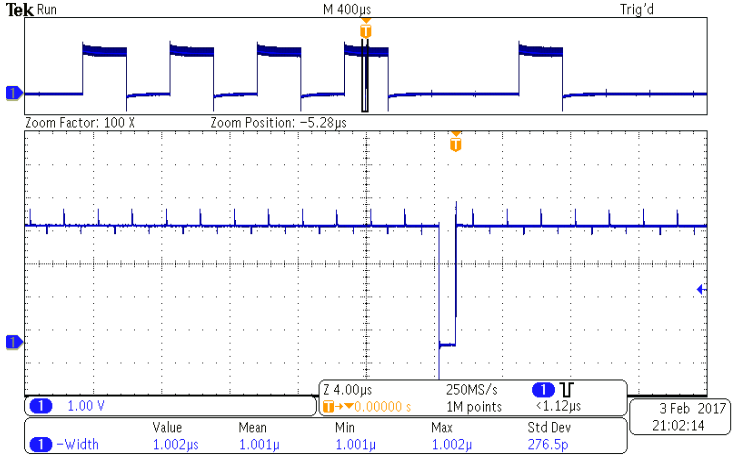
\includegraphics[width=0.87\textwidth]{images/05-zadani.png}

\subsection{Měření zpoždění}
Na vstupy osciloskopu přiveďte signály č. 5 a č. 6, osciloskop zasynchronizujte (můžete využít tlačítko AUTOSET). Pomocí funkce automatického měření změřte zpoždění (delay) mezi náběžnými a poté mezi sestupnými hranami těchto signálů.

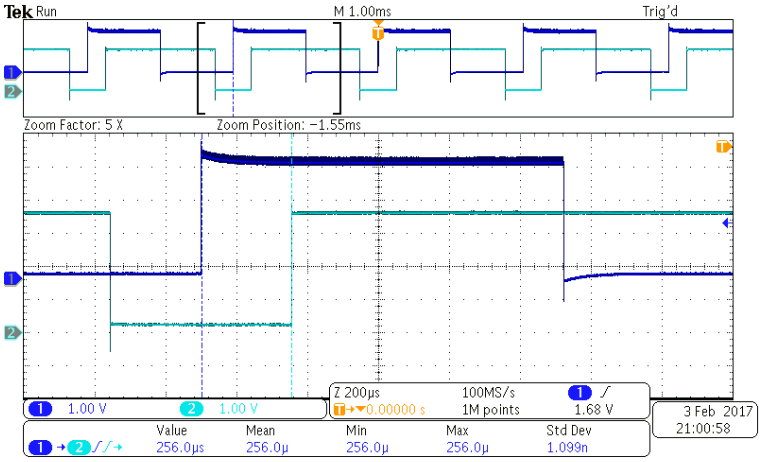
\includegraphics[width=0.87\textwidth]{images/06-zadani.png}

\subsection{Spouštění runt pulsem}
Signál č. 8 obsahuje puls s nižší napěťovou úrovní pro log.1 (pravděpodobná kolize dvou budičů, kdy jeden generuje úroveň log.1 a druhý log.0). Nastavte osciloskop tak, aby spouštěl od výskytu tohoto pulsu (runt) a poté změřte pomocí funkce automatického měření napěťovou úroveň odpovídající log. 1 u běžného i kolizního pulsu.

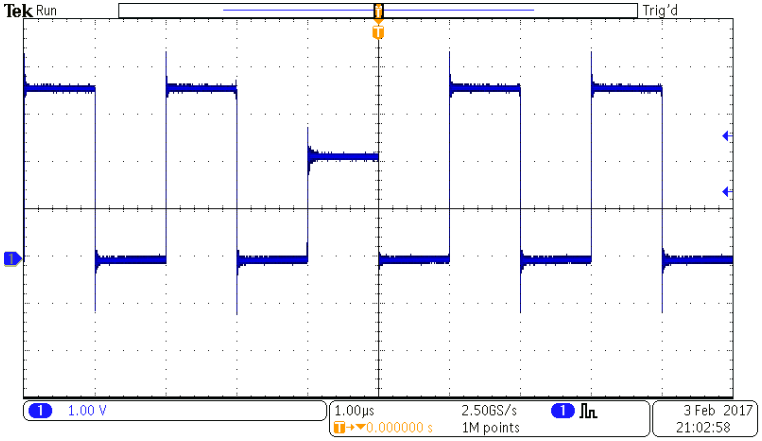
\includegraphics[width=0.87\textwidth]{images/07-zadani.png}

\subsection{Spouštění délkou hrany pulsu}
Signál č. 9 obsahuje puls s delšími hranami, než mají ostatní pulsy (degradace či nevhodná technologie jednoho z budičů na sběrnici). Nastavte osciloskop tak, aby spouštěl od výskytu tohoto pulsu a poté změřte pomocífunkce automatického měření rychlost náběžné a sestupné hrany standardního i degradovaného pulsu.

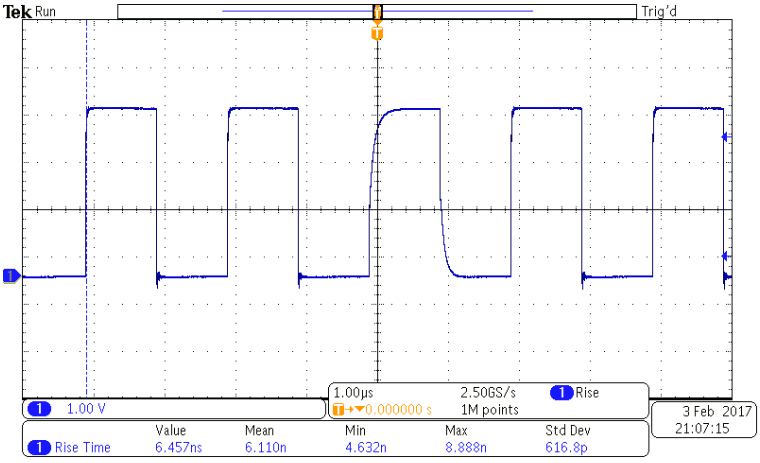
\includegraphics[width=0.87\textwidth]{images/08-zadani.png} 	% Information about the purpose of this project
%!TEX root=../protocol.tex	% Optional

\section{Naměřené hodnoty}
\subsection{Nastavení pulsu}
\begin{figure}[h]
\centering
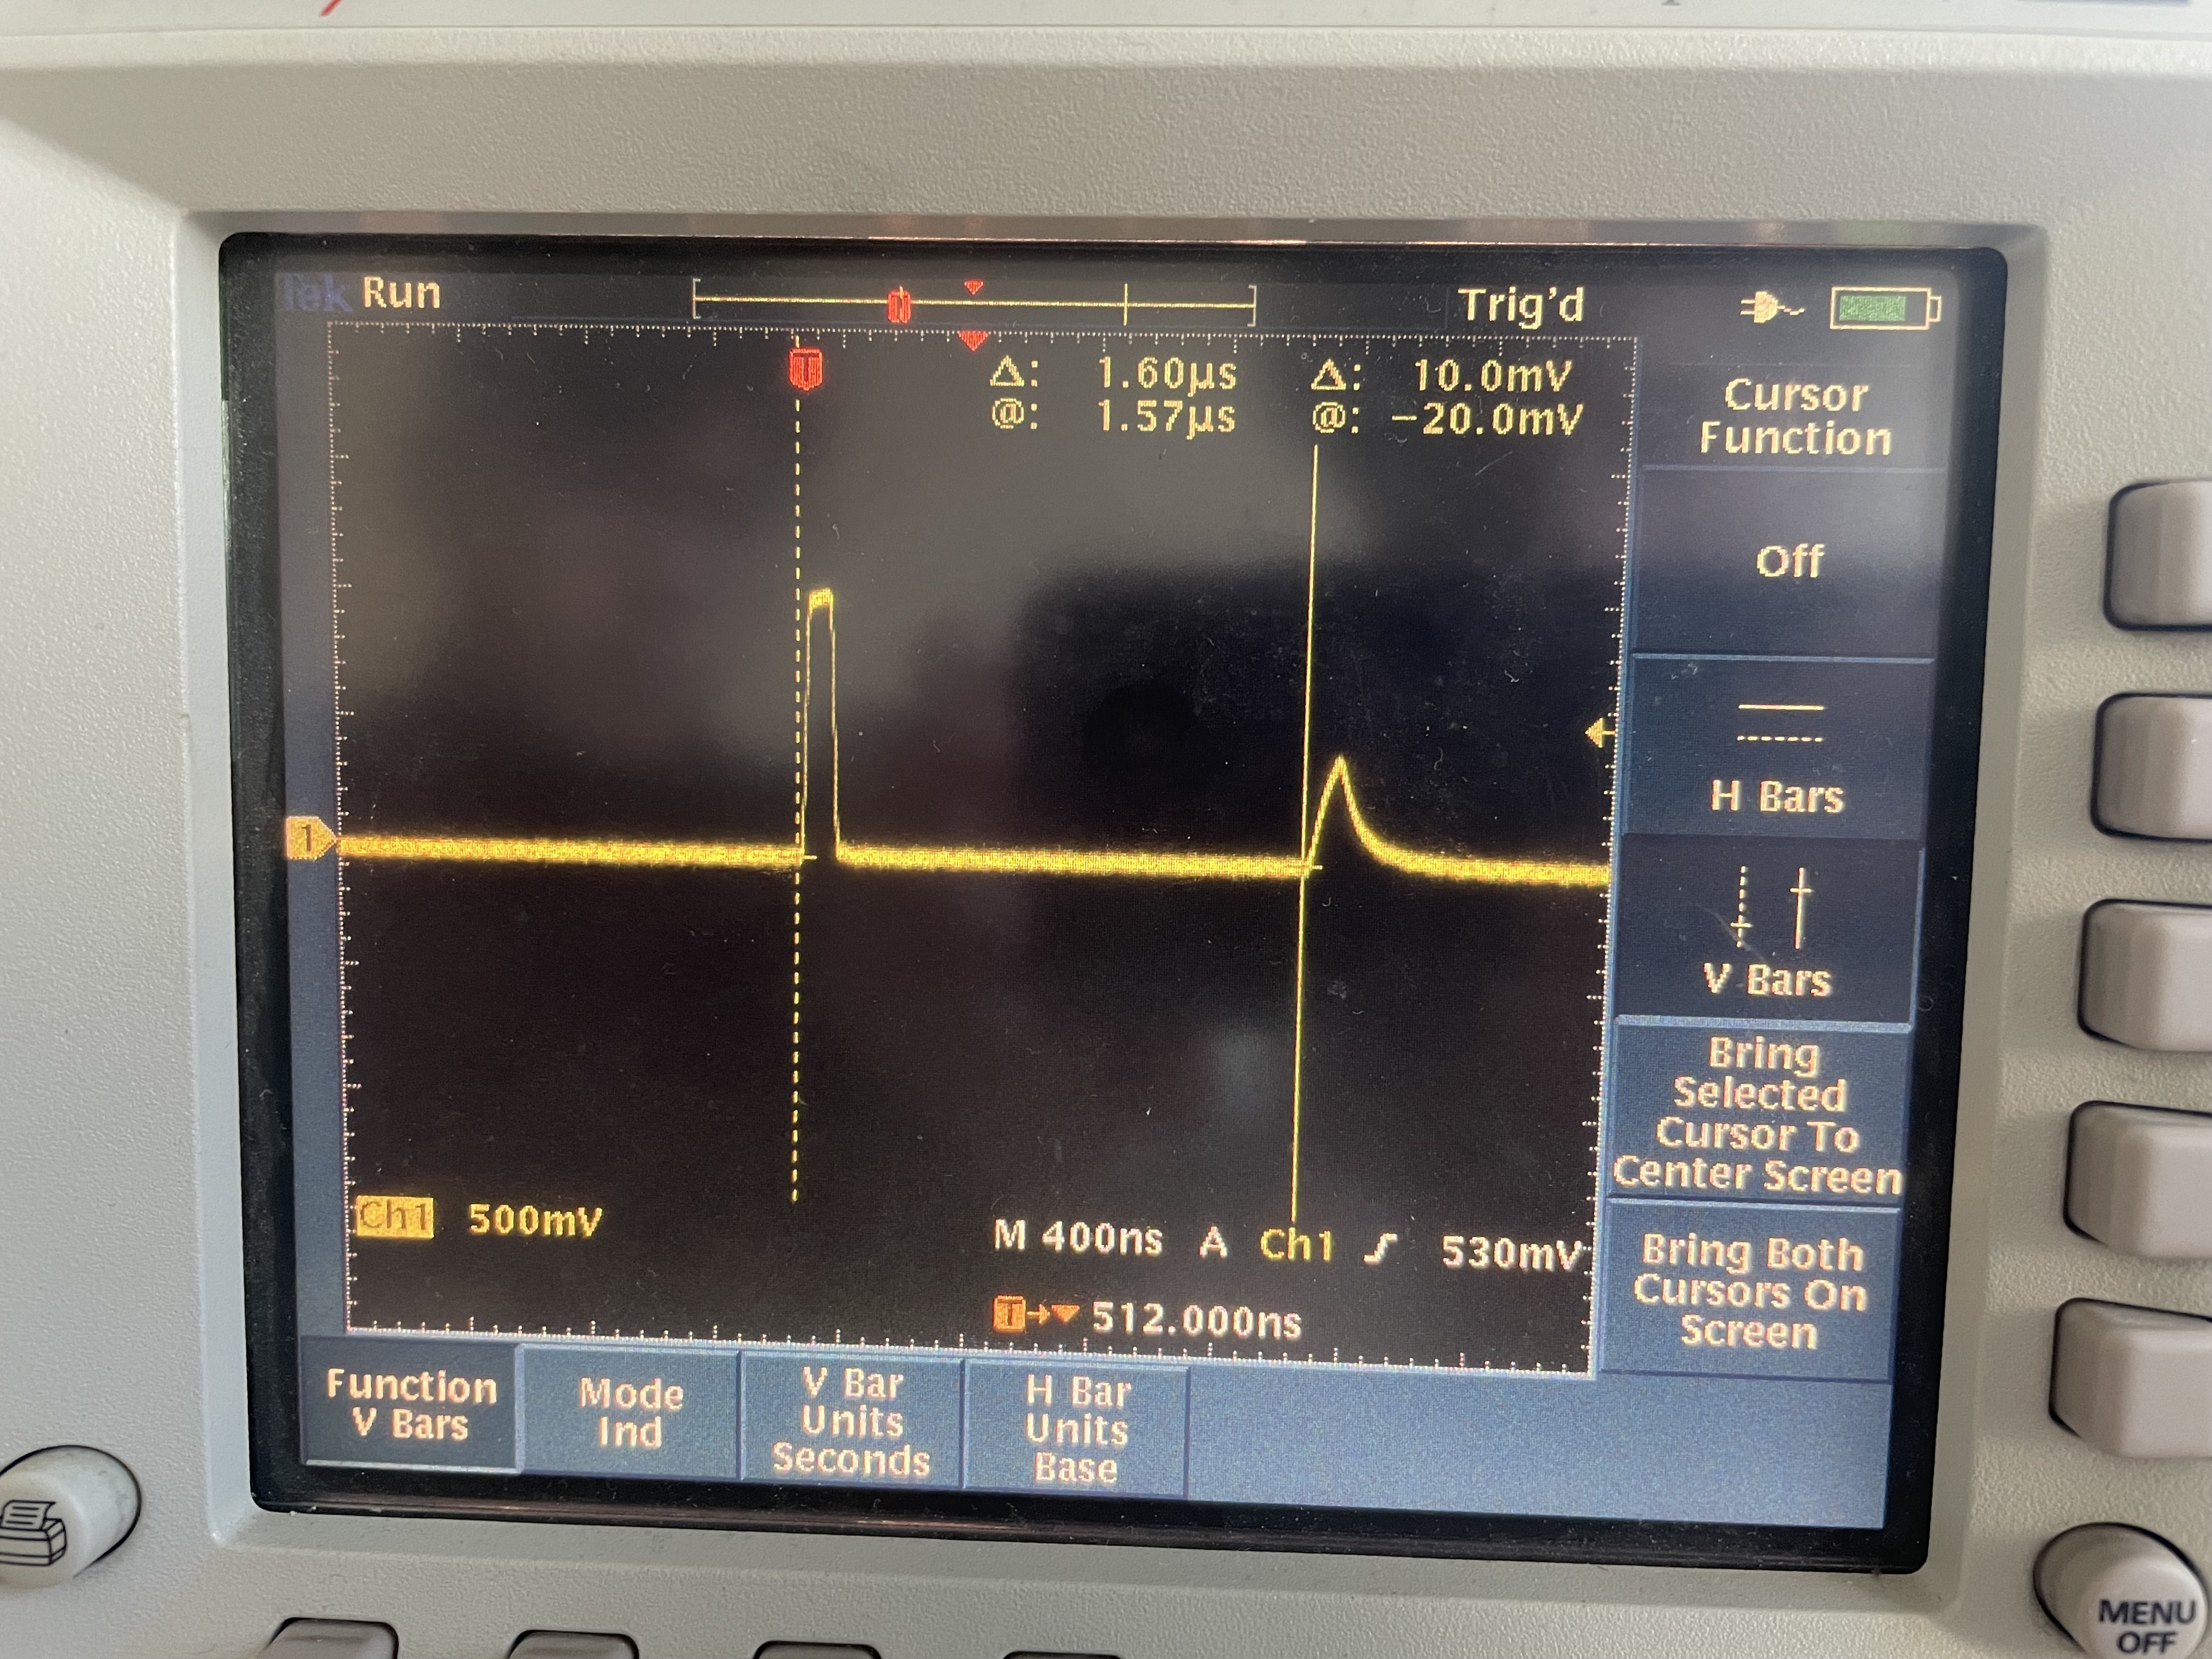
\includegraphics[width=14cm]{images/obr_1.jpg}
\caption{Používaný signál}
\label{fig:5}
\end{figure}

Z toho jsme určili t$=1,6 \cdot 10^{-6}$ s.
\newpage
\subsection{Činitel odrazu na konci vedení}
Nechť činitel odrazu \[\rho_b = \frac{R - Z}{R + Z}\] \\ a mějme $Z=50$ $\Omega$. Pak:

\begin{table}
    \centering
    \caption{Spočítané hodnoty činitele odrazu}
    \begin{tabular}{|c|c|}
       \hline
       R / $\Omega$ & $\rho_b$ / $\Omega$\\
       \hline
       0  & -1\\
       \hline
       25  & -$\frac{1}{3}$\\
       \hline
       50  & 0\\
       \hline
       100  & $\frac{1}{3}$\\
       \hline
       $\infty$ & 1\\
       \hline
    \end{tabular}
    \label{tab:1}
\end{table}
\subsection{Měření délky vedení}
Délka vedení je \[l = 0,65 \cdot c \cdot t \cdot \frac{1}{2}\ \dot{=}\ 0,65 \cdot 3 \cdot 10^{-8} \cdot 1,6 \cdot 10^{-6} \cdot \frac{1}{2}\  \dot{=}\  156\ m.\]
\subsection{Měření impedance vedení}
K odrazu nedochází při odporu $R = 50,3\ \Omega$.
\newpage
\subsection{Data impedančního přizpůsobení}
\begin{figure}[h]
\centering
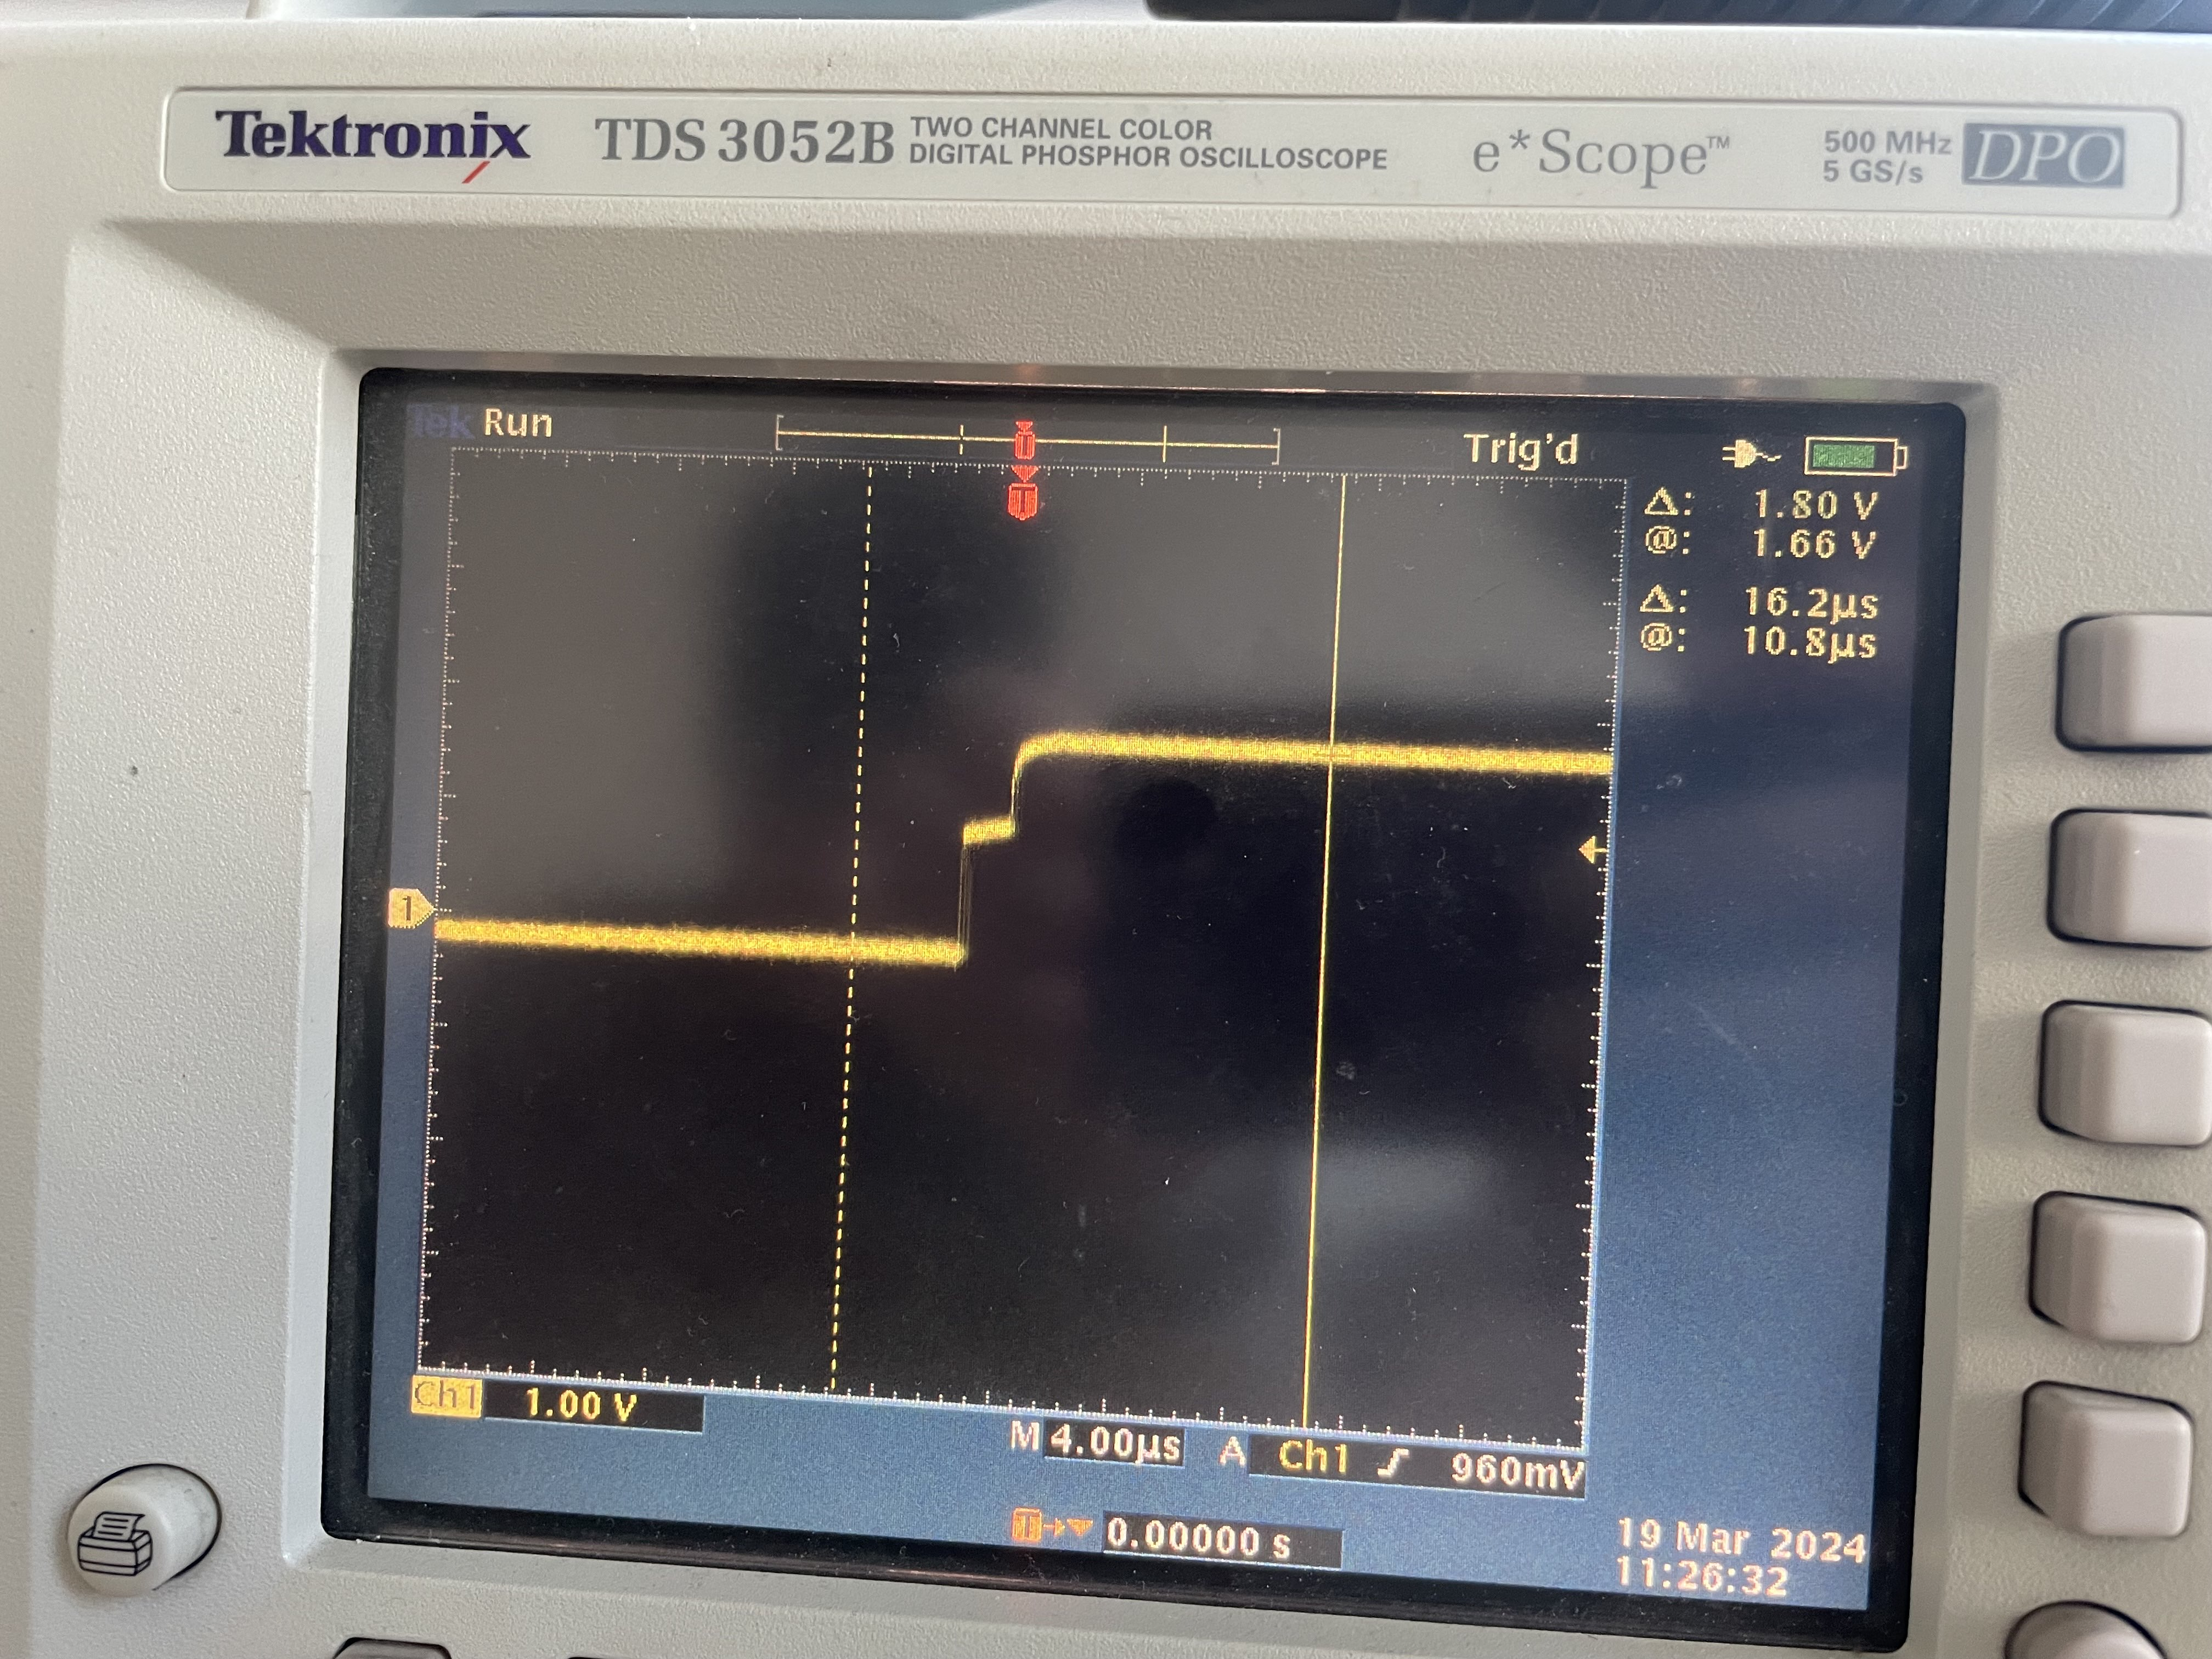
\includegraphics[width=13cm]{images/obr_4.jpg}
\caption{Průběh signálu}
\label{fig:6}
\end{figure}
Signál se nejspíše z části odrazí na začátku vedení, což se zobrazí jako meziskok na osciloskopu.
\section{Zhodnocení}
Během měření jsme si ukázali možnosti využití impedančního přizpůsobení pro detekce různých vad na metalickém vedení. Všechna měření jsme stihli v požadovaném čase i s ohledem na různé pokusy nad rámec zadání.
 % Solution for the given tasks and their documentation
% \glsaddall 		% Add all glossary entries to printglossaries
\end{document}
